\documentclass[12pt,a2paper,landscape,innermargin=20mm]{tikzposter}

\useblockstyle{Envelope}
\usebackgroundstyle{VerticalGradation}
\usecolorstyle{Spain}
\usetitlestyle{Envelope}

\usepackage[utf8]{inputenc}
\usepackage{amsmath}
\usepackage{amsfonts}
\usepackage{amssymb}
\usepackage{blindtext}
\usepackage{layout}
\usepackage{url}

\author{David Pérez, Ander Raso}
\title{\textbf{Aplicaciones de la Minería de Datos en Medicina}}
\date{}

\begin{document}

\maketitle

\begin{columns}

\column{0.35}
\block{ENUNCIADO}{
%Introducción
%Enunciado del problema a resolver
Para ilustrar la aplicación de la minería de datos en la sanidad vamos a explicar un caso ficticio presentado en el Artículo "Data Mining Applications in Healthcare"\cite{A_DMAHC}.

Supongamos que como parte de su programa del cuidado de la salud, HealthOrg (una organización ficticia) está interesada en \textbf{averiguar como ciertas variables se relacionan con el desarrollo de la diabetes}. El propósito de esta aplicación de minería de datos será identificar individuos con alto riesgo para notificarles adecuadamente.
}

\column{0.25}
\block{INSTANCIAS}{
%Origen de los datos
%¿Cómo vienen caracterizadas las instancias? ¿A través de cuántas características o atributos se describen las instancias?
%¿Cuál es la variable "clase" que se quiere determinar?
HealthOrg dispone de un conjunto de datos que contienen siete atributos de interés: género, edad, BMI (Body Max Index/índice de Masa Corporal), WHR (Waist Hip Ratio/Índice Cintura Cadera), fumador, número de veces que el paciente se ejercita por semana y si {es diabético}. Este último dato es la calse que se quiere llegar a predecir.

Se disponen de \textbf{2040 instancias}. 262 (12,78\%) casos de diabéticos y 1778 (87,22\%) de no diabéticos.
}

\column{0.4}
\block{RESULTADOS}{
%Resultados del experimento
%Observaciones
%Variables predictoras

Las cuatro variables más discriminantes fueron, de mayor a menor: \textbf{la edad, el BMI, el WHR y la cantidad de ejercicio semanal.}

Los individuos mayores de 50 años tienen significantemente más riesgo de diabetes.

Los casos con edad menor a 50 y con un BMI menor de 28,52 tienen muy poco riesgo (una probabilidad de solo 3,29\%). Incrementar el BMI está asociado con incrementar el riesgo de diabetes. Para los indivuos mayor de 50 años con un BMI mayor de 24,51 su riesgo es del 75,14\%.

Incrementar el WHR está asociado a un mayor riesgo de diabetes. Individuos mayores de 50 años con un BMI mayor de 24,31 y un WHR mayor de 0,83 tienen un riesgo del 86,33\%.
}

\end{columns}

\begin{columns}

\column{0.4}
\block{IMG1}{
\begin{center}
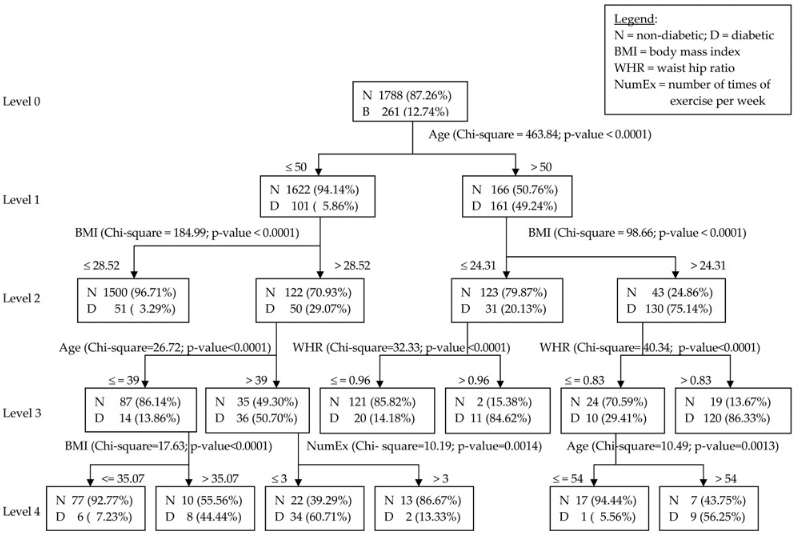
\includegraphics[scale=0.55]{fig/arbol_decision.png}
\linebreak
Figure 1: árbol de decisión\cite{A_DMAHC}
\end{center}
}

\column{0.35}
\block{IMG2}{
\begin{center}
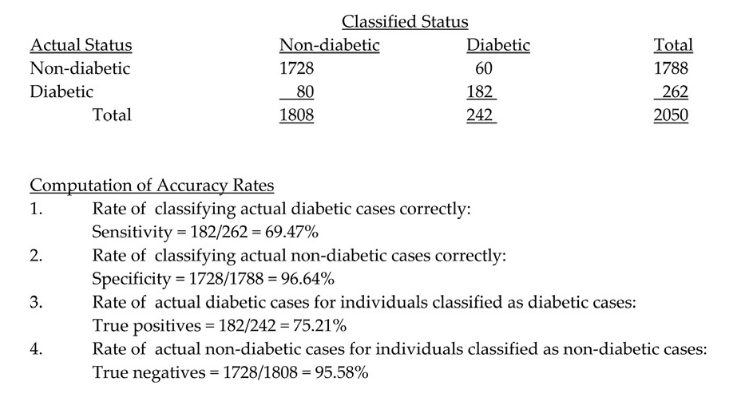
\includegraphics[scale=0.7]{fig/tabla_clasifiacion.png}
\linebreak
Figure 2: tabla de clasificación\cite{A_DMAHC}
\end{center}
}

\column{0.25}
\block{CONCLUSIONES}{
%¿Qué interés tiene en este problema utilizar minería de datos? (¿no hay expertos?, ¿hay demasiados datos?)
%Posibilidad de automatización gracias a abundancia de datos.
Utilizar la minería de datos ha sido de interés ya que se ha podido crear un modelo predictor de diabetes y se ha averiguado que variables influyen en su aparición. Sabiendo esto HealthOrg puede crear campañas de promoción de la salud para educar a la población de que BMI y WHR altos son factores de riesgo para sufrir diabetes.

Las aplicaciones de minería de datos pueden beneficiar a la sanidad. Sin embargo, hay varias limitaciones. La minería de datos se ve limitada por la accesibilidad de los datos, porque estos se encuentran diseminados en diferentes lugares, como la administración, clínicas, laboratorios y más. Por lo tanto, los datos deben ser recolectados e integrados antes de que se pueda realizar la minería.
}

\end{columns}

\block{}{
\bibliography{bib/bib} 
\bibliographystyle{ieeetr}
%http://citeseerx.ist.psu.edu/viewdoc/download?doi=10.1.1.92.3184&rep=rep1&type=pdf
}

\end{document}
